	\section{پیاده‌سازی و نتایج}

همان طور که در 
\cite{wang2019easy}
بیان شده است در روش 
\lr{\textit{EasyTL}}
باید دو قسمت زیر را پیاده‌سازی کنیم:
\begin{enumerate}
	\item{\lr{\textit{Intra-domain programming}}}
	\item {\lr{\textit{Intra-domain alignment}}}
\end{enumerate}

بخش 
\lr{\textit{Intra-domain programming}}
شامل 3 مرحله نیز می‌باشد:
\begin{enumerate}
	\item{	
		محاسبه‌ی بردار مراکز کلاس‌های دامنه‌ی مبدا $h_c$: این قسمت در تابع 
		\lr{\textbf{\textit{get\_class\_center(Xs, Ys)}}}
		پیاده‌سازی شده است.}
	\item{
		محاسبه‌ی ماتریس فاصله $D$: این قسمت در تابع 
		\lr{\textbf{\textit{get\_distance\_matrix(Xt, class\_center)}}}
		پیاده‌سازی شده است.}
	\item{
		بدست آوردن ماتریس احتمال $M$ با استفاده از معادله‌ی فلان و بدست آوردن برچسب دامنه هدف: این قسمت در تابع 
	\lr{\textbf{\textit{solve\_LP(C, nt, Dcj)}}}
	پیاده‌سازی شده است.}  
\end{enumerate}

سپس از نتایج این سه تابع استفاده می‌کنیم و آن‌ها را در تابع 
\lr{\textbf{\textit{intra\_domain\_programming(Xs, Ys, Xt, Yt)}}}
با هم ترکیب می‌کنیم.در بخش 
\lr{\textit{Intra-domain alignment}}
کافی است تنها معادله‌ی فلان را پیاده‌سازی کنیم. بدین منظور از تابع 
\lr{\textbf{\textit{intra\_domain\_alignment(Xs, Xt)}}}
استفاده می‌کنیم.

روش
\lr{\textit{EasyTL}}
را می‌توانیم به دو صورت اجرا کنیم. در یک حالت فضای دامنه‌ها را بایکدیگر تراز نمی‌کنیم و فقط بخش 
\lr{\textit{Intra-domain programming}}
را اجرا می‌کنیم و در حالت دیگر ابتدا فضای دامنه‌ها را به یکدیگر تراز می‌کنیم و سپس طبقه‌بند موجود در دامنه مبدا را به دامنه هدف منتقل می‌کنیم. این روش را بر روی 4 مجموعه‌داده آزمایش می‌کنیم و نتایج را مقایسه می‌کنیم. این 4 مجموعه داده به شرح زیر هستند:
\begin{enumerate}
	\item {
		\lr{\textit{Amazon Review}}
		یک مجموعه داده تجزیه و تحلیل احساسات است که شامل بررسی‌های مثبت و منفی چهار نوع محصول است: لوازم آشپزخانه ، دی وی دی، الکترونیک و کتاب}

	\item{
		\lr{\textit{Office-Caltech}}
		شامل 10 کلاس از تصاویر در آمازون، DSLR، وب کم و Caltech است.
	}
	\item {
		\lr{\textit{Image-CLEF DA}}
		شامل 12 دسته تصویر متعلق به 3 حوزه است: Caltech ، ImageNet  و Pascal.
	}

	\item {
		\lr{\textit{Office-Home}}
		شامل 15،500 تصویر از 65 دسته از 4 حوزه Art، Clipart ، Product و دنیای واقعی است.
	}
\end{enumerate}

\begin{figure}
	\centering
	\begin{subfigure}[b]{0.2\textwidth}
		\centering
		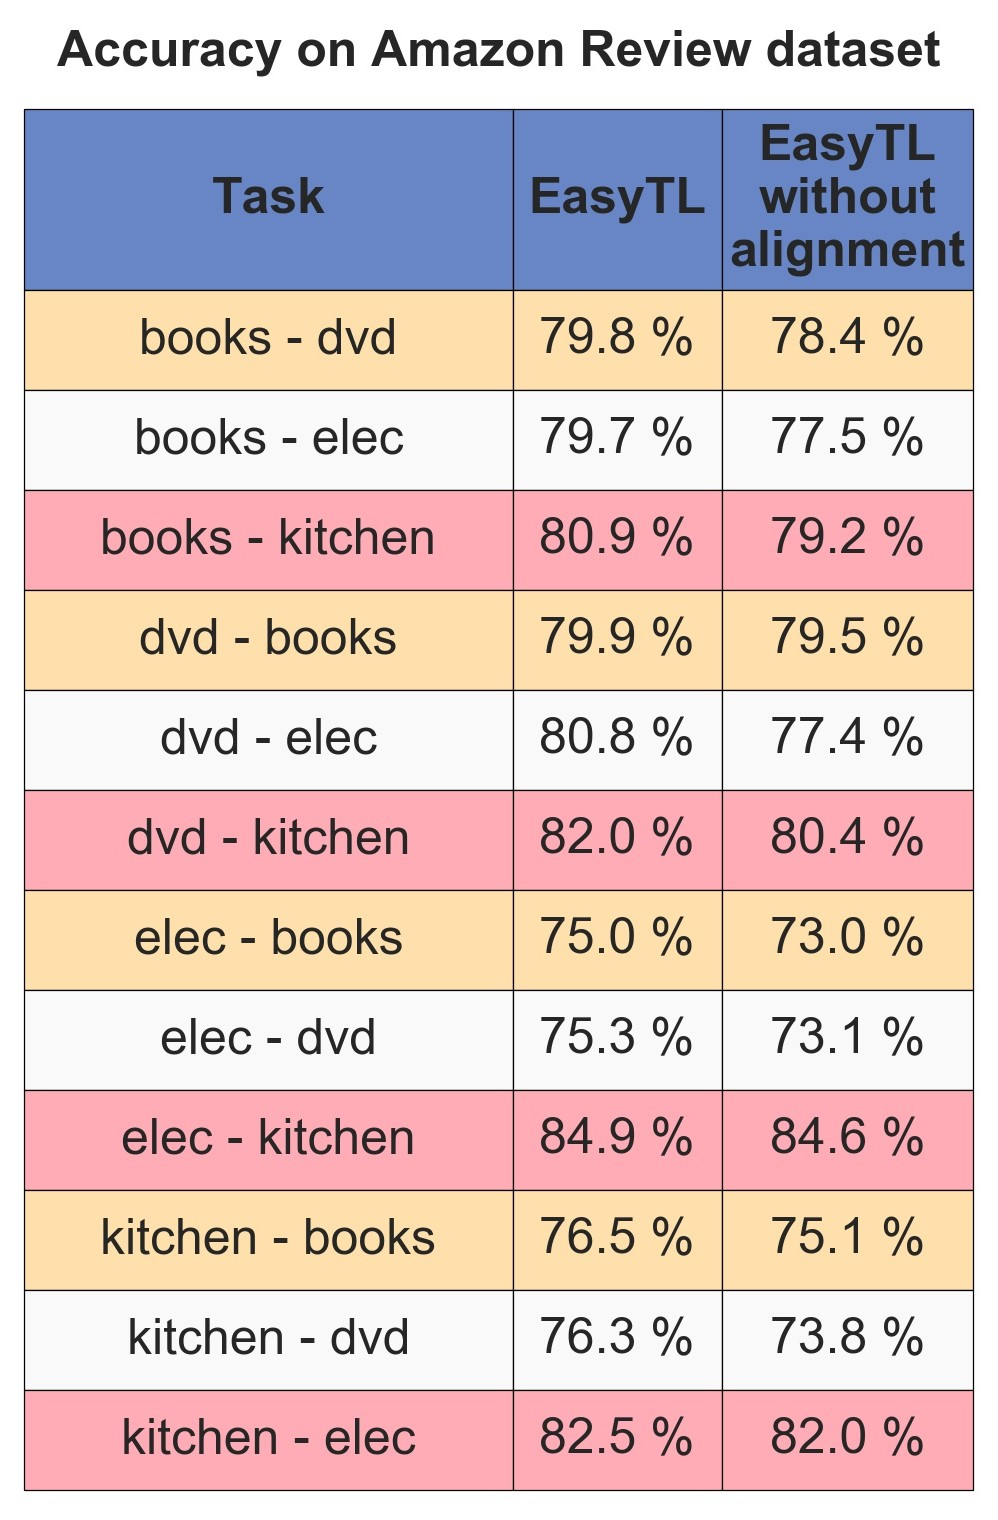
\includegraphics[width=0.85\linewidth]{images/1_1.jpg}
		\caption{}
	\end{subfigure}%
	\begin{subfigure}[b]{0.4\textwidth}
		\centering
		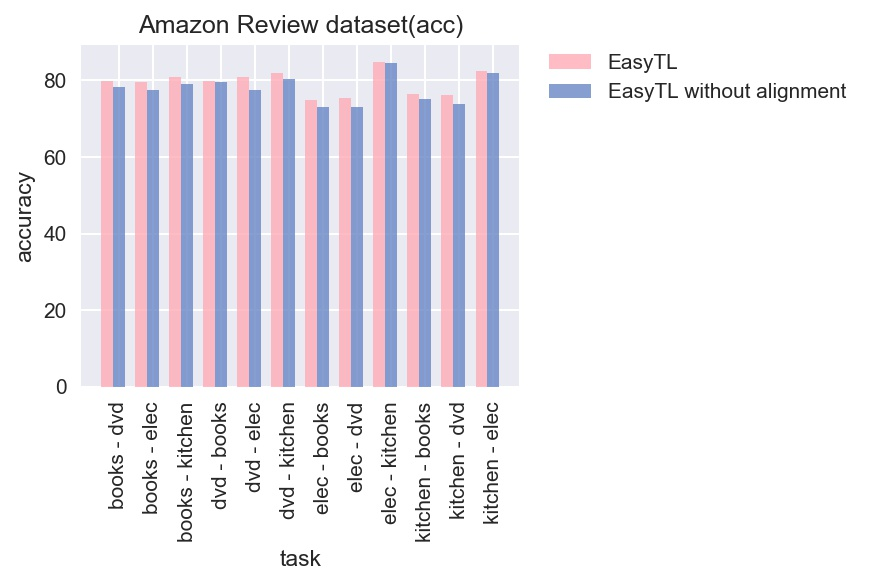
\includegraphics[width=\linewidth]{images/1_2.jpg}
		\caption{}
	\end{subfigure}%
	\begin{subfigure}[b]{0.4\textwidth}
		\centering
		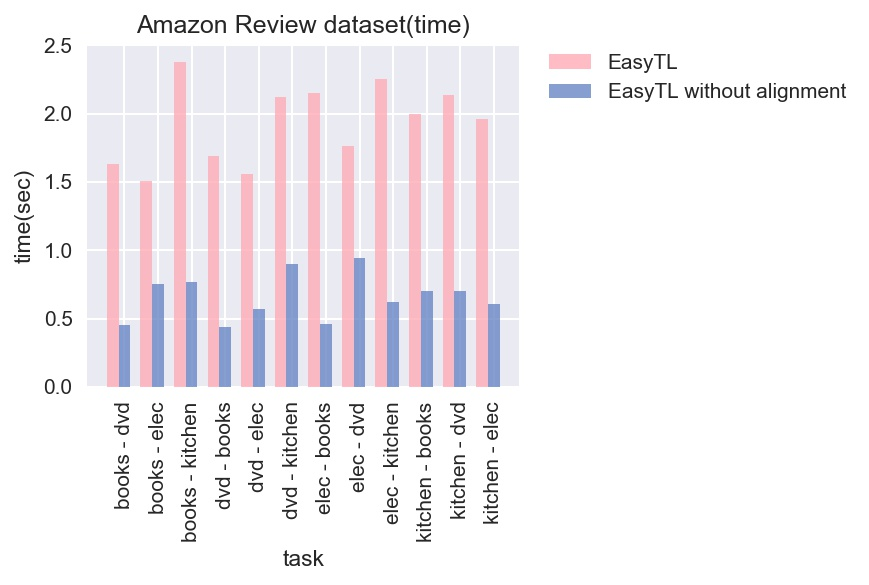
\includegraphics[width=\linewidth]{images/1_3.jpg}
		\caption{}
	\end{subfigure}%
	\caption{
		نتایج روش
		 \lr{\textit{EasyTL}}
		 بر روی مجموعه داده
		\lr{\textit{Amazon Review}}
	}
	\label{fig:1}
\end{figure}

\begin{figure}
	\centering
	\begin{subfigure}[b]{0.3\textwidth}
		\centering
		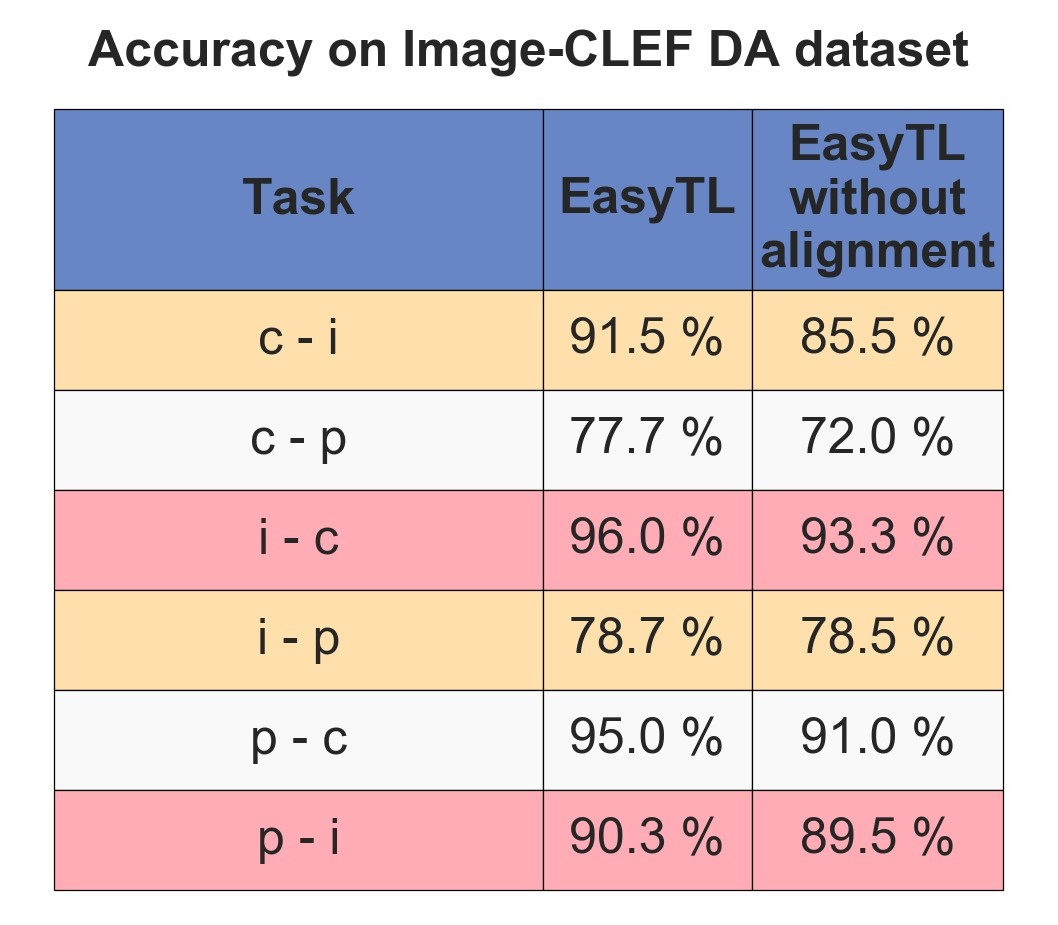
\includegraphics[width=\linewidth]{images/2_1.jpg}
		\caption{}
	\end{subfigure}%
	\begin{subfigure}[b]{0.35\textwidth}
		\centering
		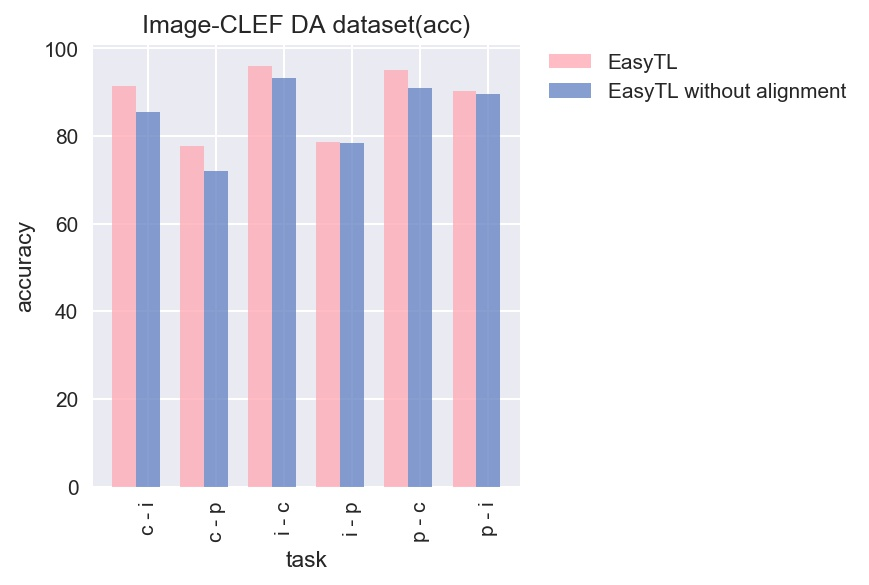
\includegraphics[width=\linewidth]{images/2_2.jpg}
		\caption{}
	\end{subfigure}%
	\begin{subfigure}[b]{0.35\textwidth}
		\centering
		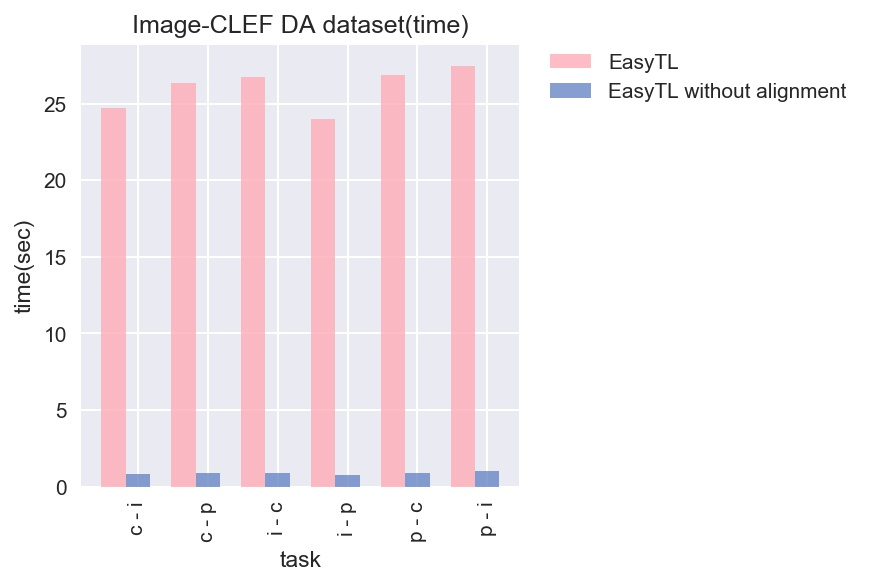
\includegraphics[width=\linewidth]{images/2_3.jpg}
		\caption{}
	\end{subfigure}%
	\caption{
		نتایج روش
		\lr{\textit{EasyTL}}
		بر روی مجموعه داده
		\textit{\lr{Image-CLEF DA }}
	}
	\label{fig:2}
\end{figure}

\begin{figure}
	\centering
	\begin{subfigure}[b]{0.25\textwidth}
		\centering
		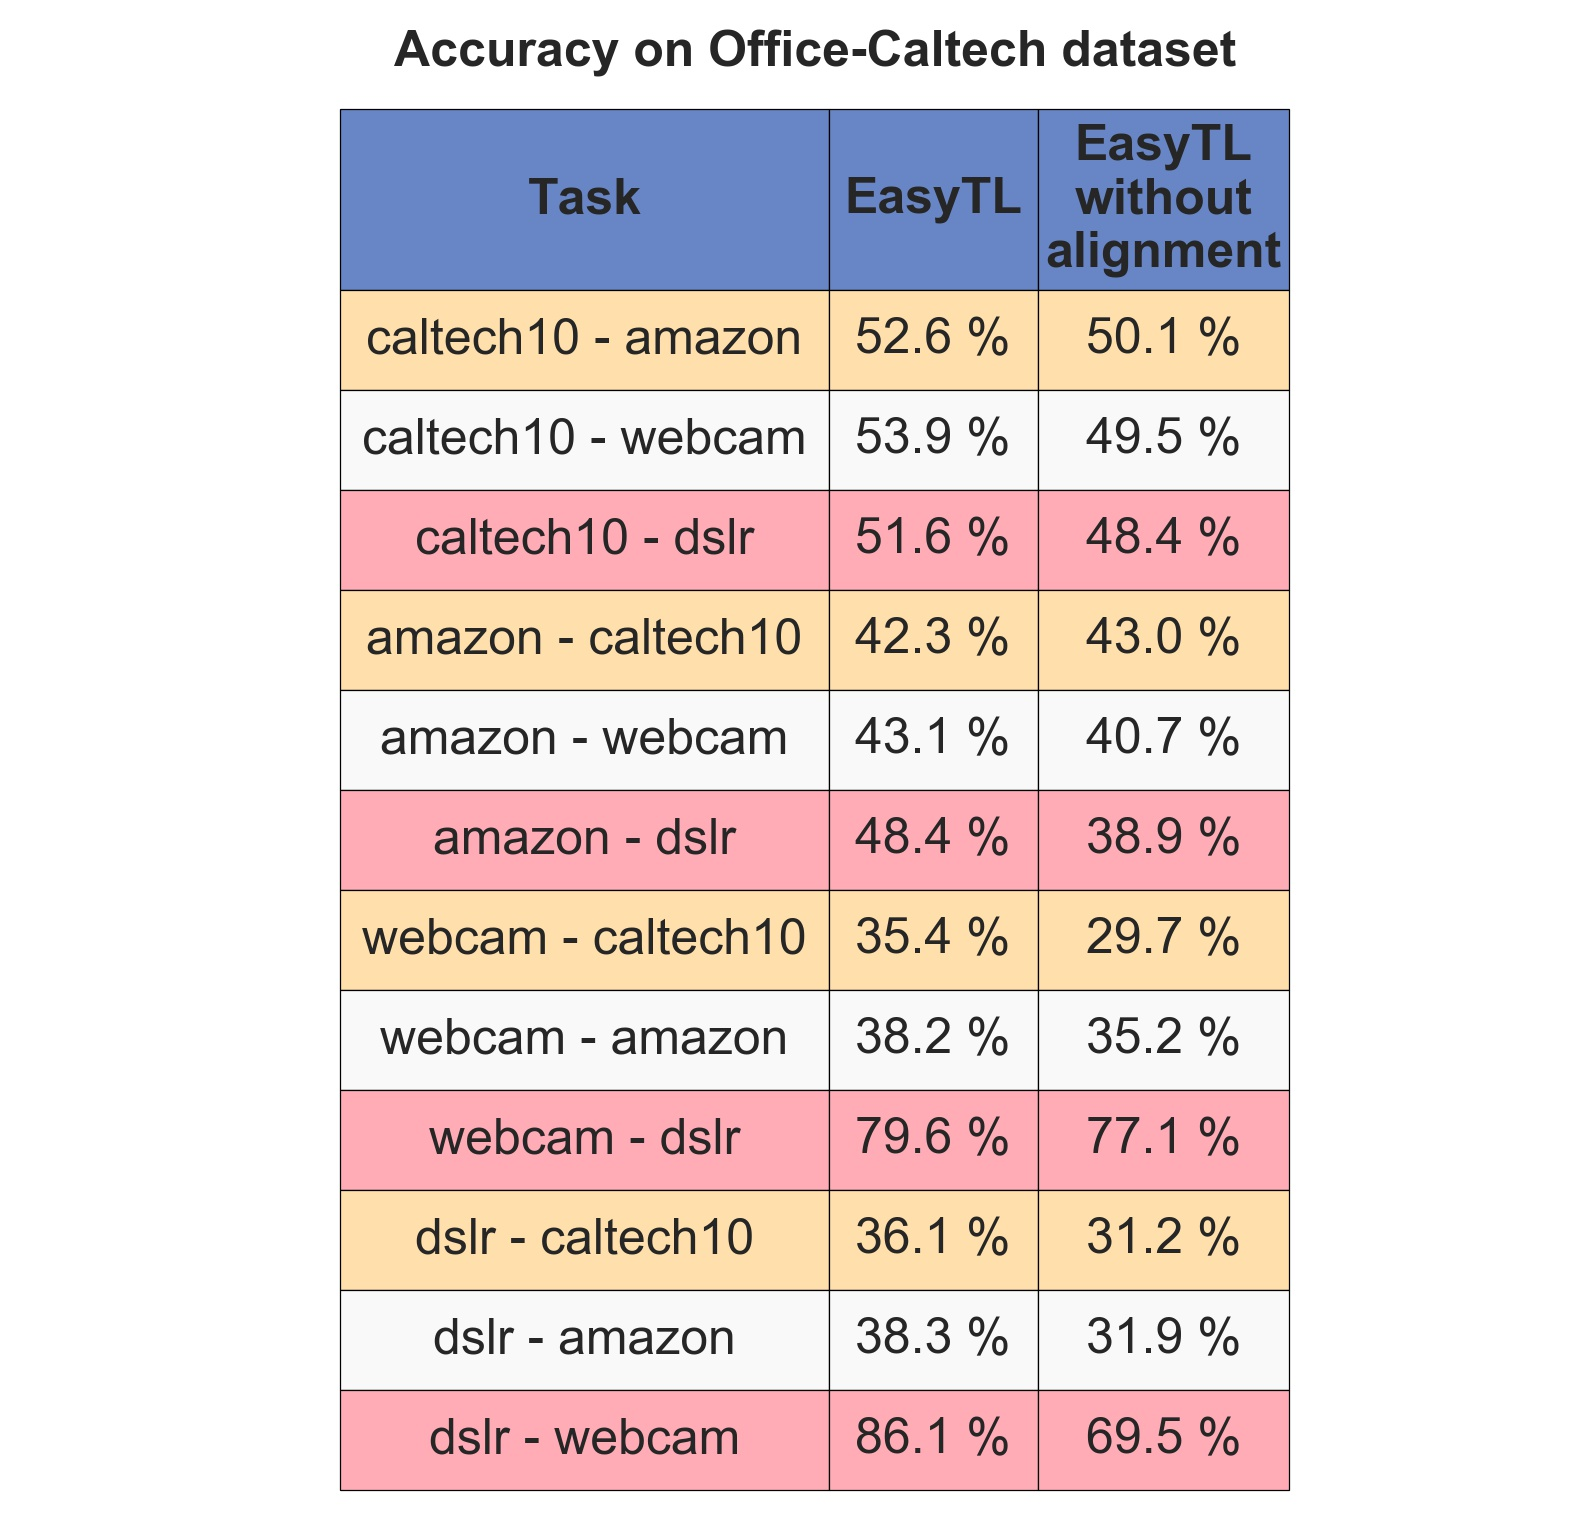
\includegraphics[width=\linewidth]{images/3_1.jpg}
		\caption{}
	\end{subfigure}%
	\begin{subfigure}[b]{0.35\textwidth}
		\centering
		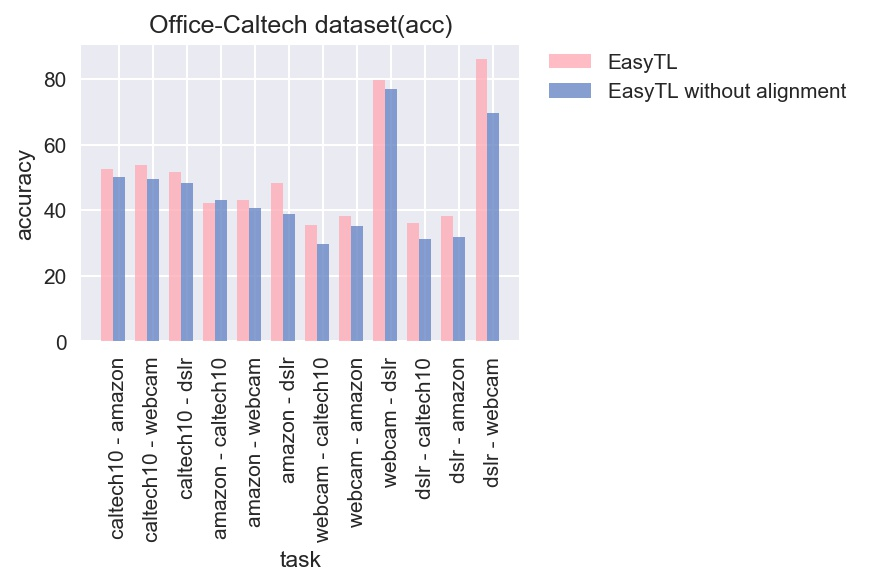
\includegraphics[width=\linewidth]{images/3_2.jpg}
		\caption{}
	\end{subfigure}%
	\begin{subfigure}[b]{0.35\textwidth}
		\centering
		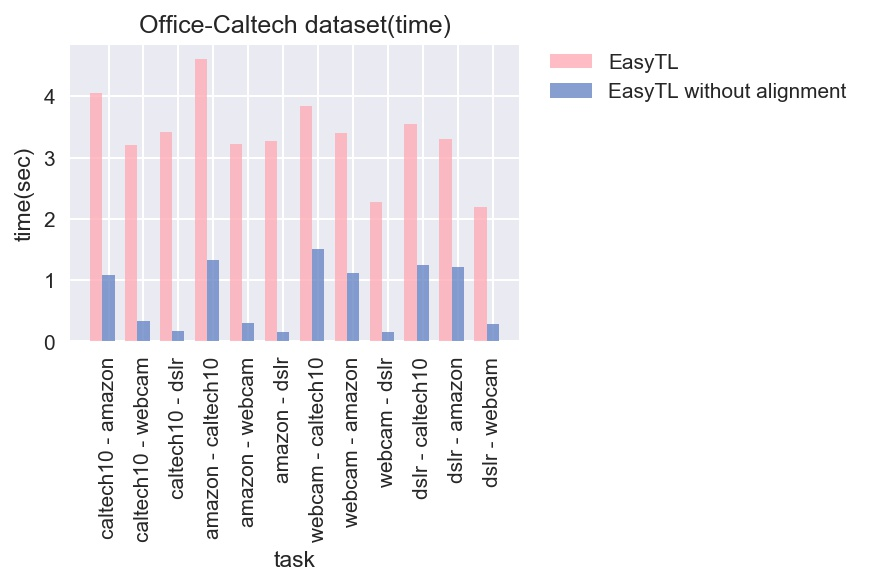
\includegraphics[width=\linewidth]{images/3_3.jpg}
		\caption{}
	\end{subfigure}%
	\caption{
		نتایج روش
		\lr{\textit{EasyTL}}
		بر روی مجموعه داده
		\textit{\lr{Office-Caltech}}
	}
	\label{fig:3}
\end{figure}

\begin{figure}
	\centering
	\begin{subfigure}[b]{0.25\textwidth}
		\centering
		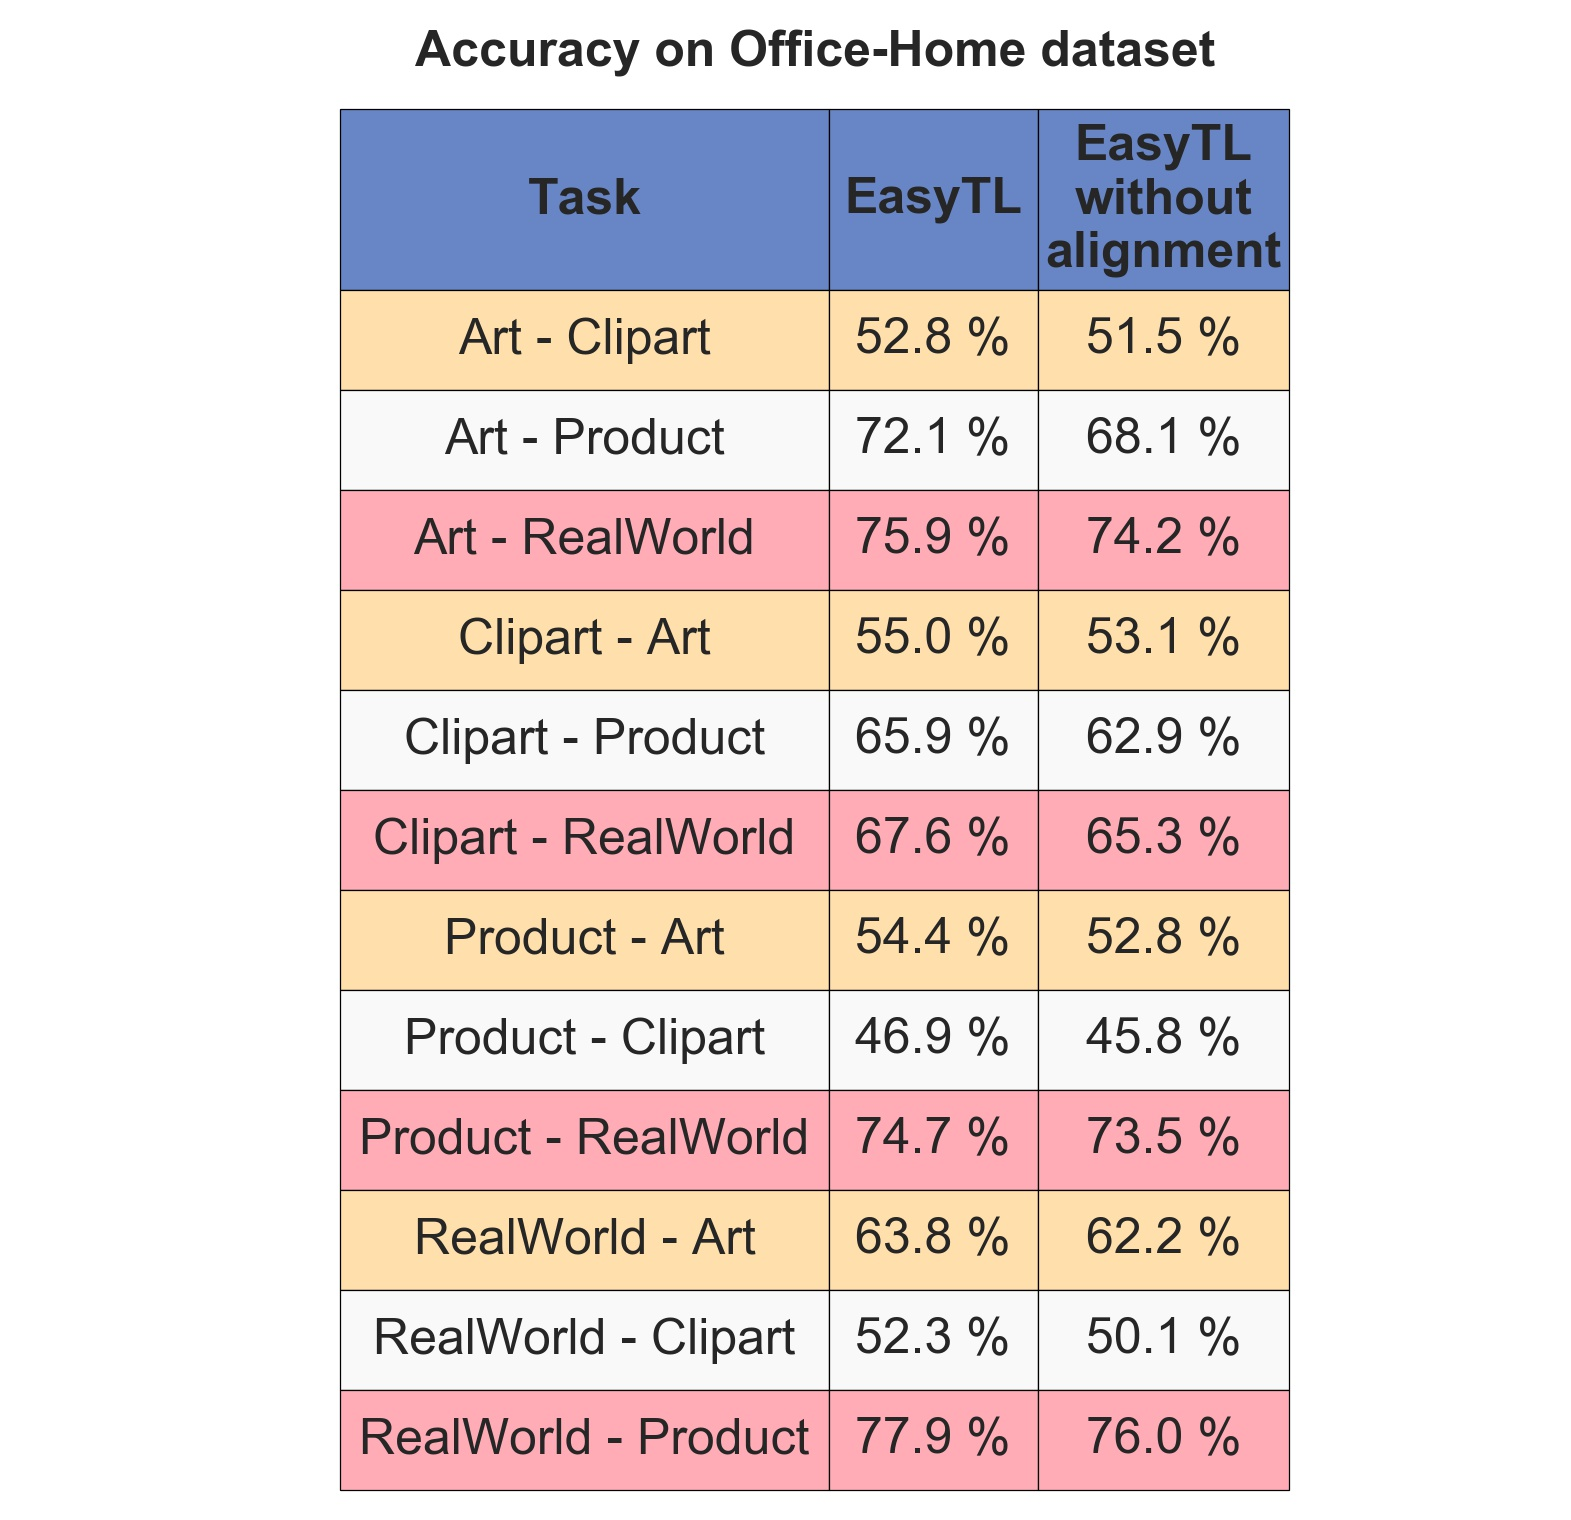
\includegraphics[width=\linewidth]{images/4_1.jpg}
		\caption{}
	\end{subfigure}%
	\begin{subfigure}[b]{0.35\textwidth}
		\centering
		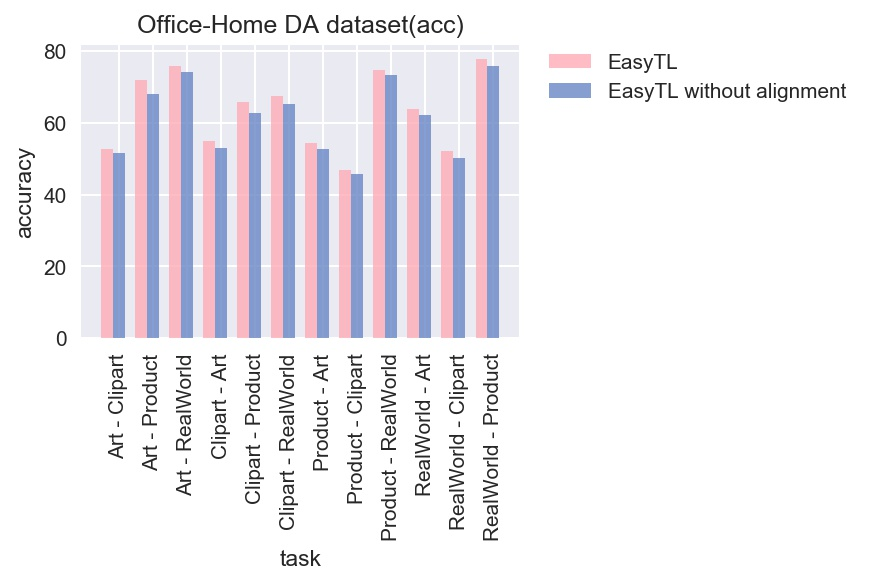
\includegraphics[width=\linewidth]{images/4_2.jpg}
		\caption{}
	\end{subfigure}%
	\begin{subfigure}[b]{0.35\textwidth}
		\centering
		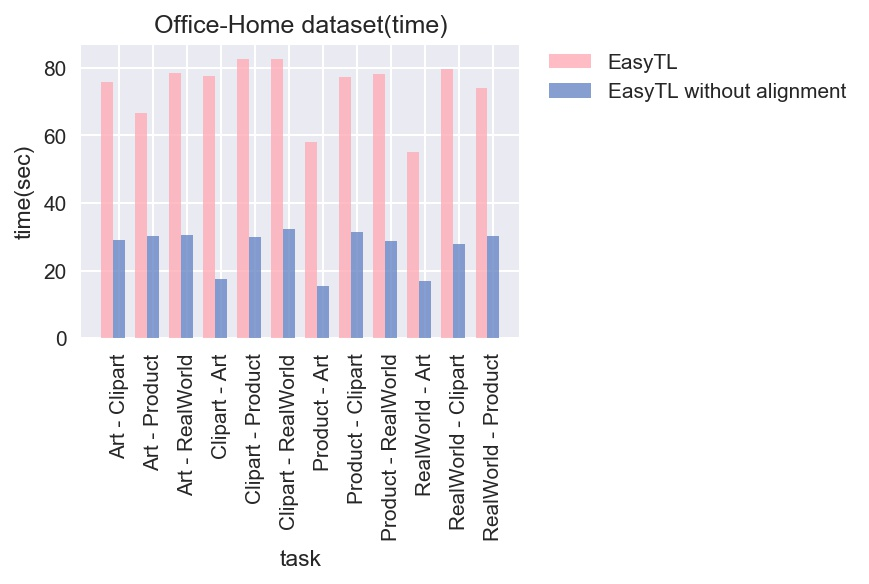
\includegraphics[width=\linewidth]{images/4_3.jpg}
		\caption{}
	\end{subfigure}%
	\caption{
		نتایج روش
		\lr{\textit{EasyTL}}
		بر روی مجموعه داده
		\textit{\lr{Office-Home}}
	}
	\label{fig:4}
\end{figure}

نتایج اجرای روش
\lr{EasyTL}
را بر روی 4 تا مجموعه‌داده ذکر شده را در شکل‌های
\ref{fig:1}
،
\ref{fig:2}
،
\ref{fig:3}
و
\ref{fig:4}
می‌توانید مشاهده کنید. از مقایسه‌ی شکل‌های قسمت (آ) در تمامی شکل‌های 
\ref{fig:1}
،
\ref{fig:2}
،
\ref{fig:3}
و
\ref{fig:4}
 با نتایج مقاله به این نتیجه می‌رسیم که دقت‌هایی که بدست آوردیم کاملا مطابق با دقت‌های مقاله است. از شکل‌های قسمت (ب) و (ج) در تمامی شکل‌های
\ref{fig:1}
،
\ref{fig:2}
،
\ref{fig:3}
و
\ref{fig:4}
می‌توانیم به یک نتیجه‌گیری کلی برسیم و آن این است که دقت در حالتی که روش 
\lr{\textit{EasyTL}}
 را بدون تراز کردن اجرا می‌کنیم با حالتی که تراز کردن را در نظر نمی‌گیریم تفاوت چندانی ندارد اما از لحاظ زمان و سرعت روش 
 \lr{\textit{EasyTL}}
 بدون تراز کردن بسیار سریعتر است و نیاز به زمان کمتری دارد. بنابراین در کاربردهایی که دقت برای ما از اهمیت بالایی برخوردار است می‌توانیم از روش 
 \lr{\textit{EasyTL}}
 با تراز کردن استفاده کنیم و در کاربردهایی که سرعت برای ما مهم است روش 
 \lr{\textit{EasyTL}}
  را بدون تراز کردن استفاده کنیم. به عبارت دیگر در اینجا با یک مصالحه‌ای رو به رو هستیم که با توجه به کاربرد باید تصمیم بگیریم که از کدام روش استفاده کنیم. 
  
  